% Unit 124 English translation of chapter9.tex, lines 818--950.
% Source: Methods of Algebra, Volume 2, commit
% 9a5803ff77dd3257484cb177f851a73770a59dd3 (CC BY 4.0).
% stable-unit-id: o014.aljabr2.chapter9.duality-examples-a
% Coverage: Section 9.3, from vector spaces through the cobordism example.

% segment-id: o014.li2.chapter9.duality-examples-a.h001
\section{Examples of Duality}\label{sec:duality-examples}
\hypertarget{o014.aljabr2.chapter9.duality-examples-a}{ }
% segment-id: o014.li2.chapter9.duality-examples-a.p001
We next examine some basic examples of duality theory.

% segment-id: o014.li2.chapter9.duality-examples-a.eg001
\begin{example}\label{eg:Vect-trace}
	Consider the category $\cate{Vect}(\Bbbk)$ of vector spaces over a field
	$\Bbbk$, with its standard symmetric monoidal structure and unit
	$\munit:=\Bbbk$. This is the basic model for duality.
	Proposition~\ref{prop:dualizable-module} implies that for every
	$\Bbbk$-vector space $V$,
	% segment-id: o014.li2.chapter9.duality-examples-a.q001
	\[ V \;\text{has a dual} \iff V \;\text{is finite-dimensional}. \]
	More concretely, for an $n$-dimensional $\Bbbk$-vector space, its dual
	(with no need to distinguish left from right) is taken to be
	% segment-id: o014.li2.chapter9.duality-examples-a.q002
	\[ V^* := \Hom_{\Bbbk}(V, \Bbbk), \]
	with the corresponding morphisms
	% segment-id: o014.li2.chapter9.duality-examples-a.q003
	\[\begin{tikzcd}[row sep=tiny]
		V \otimes V^* \arrow[r, "{\mathrm{ev}}"] & \Bbbk \\
		v \otimes \check{v} \arrow[mapsto, r] & \check{v}(v)
	\end{tikzcd} \quad \begin{tikzcd}[row sep=tiny]
		\Bbbk \arrow[r, "{\mathrm{coev}}"] & V^* \otimes V \\
		1 \arrow[mapsto, r] & \sum_{i=1}^n \check{v}_i \otimes v_i.
	\end{tikzcd} \]
	Here $v_1,\ldots,v_n$ is any basis of $V$, while
	$\check v_1,\ldots,\check v_n$ is its dual basis. These definitions are a
	special case of Proposition~\ref{prop:dualizable-module}, and can also be
	verified directly without difficulty.

	\index[sym1]{Vectf@$\cate{Vect}_{\mathrm{f}}$}
	Finite-dimensional $\Bbbk$-vector spaces form a rigid category under
	$\otimes$, denoted by $\cate{Vect}_{\mathrm f}(\Bbbk)$. All operations
	involving duals reduce to the following elementary facts.
	\begin{itemize}
		\item The isomorphism
		$V^*\otimes W\simeq\Hom(\Bbbk,V^*\otimes W)\rightiso\Hom(V,W)$
		sends $\sum_i\check v_i\otimes w_i$ to the linear map
		$\sum_i\check v_i(\mathord\cdot)w_i$.
		\item The dual $f^*:W^*\to V^*$ of a morphism $f:V\to W$ is precisely
		the transpose of the linear map; the diagrammatic identity
		\eqref{eqn:f-dual-ev} says it all.
		\item Trace and dimension take values in
		$\End(\Bbbk)\simeq\Bbbk$. Since
		$\cate{Vect}_{\mathrm f}(\Bbbk)$ is symmetric, there is no need to
		distinguish left from right.
		\item Upon identifying $\End(V)$ with $V^*\otimes V$,
		% segment-id: o014.li2.chapter9.duality-examples-a.q004
		\[ \Tr\left(\sum_i\check v_i\otimes v_i\right)=
		\sum_i\check v_i(v_i) \]
		is precisely the classical trace. Likewise, $\dim V$ is the image of
		the classical dimension under the homomorphism $\Z\to\Bbbk$.
	\end{itemize}
\end{example}

% segment-id: o014.li2.chapter9.duality-examples-a.eg002
\begin{example}\label{eg:superVect-trace}
	\index{super vector space}
	Consider the symmetric monoidal category
	$\cate{Vect}^-_{\Z/2\Z}(\Bbbk)$ from Example~\ref{eg:superspace}.
	Its objects and morphisms are written, respectively, as
	$V=V_0\oplus V_1$ and $f=(f_0,f_1)$, with
	$\Bbbk=\Bbbk\oplus\{0\}$ as the unit. As in
	Example~\ref{eg:Vect-trace}, an object $V$ has a dual if and only if it is
	finite-dimensional as a $\Bbbk$-vector space; all such objects form the
	full subcategory $\cate{Vect}^-_{\Z/2\Z, f}(\Bbbk)$. If $V$ is
	finite-dimensional, its dual may be taken to be
	% segment-id: o014.li2.chapter9.duality-examples-a.q005
	\[ V^* = V^*_0 \oplus V^*_1, \quad V^*_i := \Hom_{\Bbbk}(V_i, \Bbbk), \]
	with
	% segment-id: o014.li2.chapter9.duality-examples-a.q006
	\[\begin{tikzcd}[row sep=tiny, column sep=small]
		V \otimes V^* \arrow[r, "{\mathrm{ev}}"] & \Bbbk \\
		(v_0, v_1) \otimes (\check{v}_0, \check{v}_1) \arrow[mapsto, r] & \check{v}_0(v_0) - \check{v}_1(v_1), \\
		\Bbbk \arrow[r, "{\mathrm{coev}}"] & V^* \otimes V \\
		1 \arrow[mapsto, r] & \sum_{i=1}^{n_0} \check{v}_{0,i} \otimes v_{0,i} - \sum_{i=1}^{n_1} \check{v}_{1,i} \otimes v_{1,i}.
	\end{tikzcd}\]
	Here $v_{0,1},\ldots,v_{0,n_0}$ (respectively,
	$v_{1,1},\ldots,v_{1,n_1}$) is any basis of $V_0$ (respectively, $V_1$),
	while $\check v_{0,1},\ldots,\check v_{0,n_0}$ (respectively,
	$\check v_{1,1},\ldots,\check v_{1,n_1}$) is the dual basis. The
	conditions of Definition~\ref{def:dualizable-obj} can be checked directly.
	\begin{itemize}
		\item The isomorphism
		$(V^*\otimes W)_0\simeq\Hom(\Bbbk,V^*\otimes W)
		\rightiso\Hom(V,W)$ sends $\sum_i\check v_i\otimes w_i$ to the linear
		map $\sum_i\check v_i(\mathord\cdot)w_i$, where either
		$\check v_i\in V_0^*$ and $w_i\in W_0$, or
		$\check v_i\in V_1^*$ and $w_i\in W_1$.
		\item The dual $f^*:W^*\to V^*$ of a morphism $f:V\to W$ is again the
		transpose of the linear map, applied separately to each direct summand.
		\item Trace and dimension again take values in
		$\End(\Bbbk)\simeq\Bbbk$, with no distinction between left and right.
		The trace of an endomorphism $f=(f_0,f_1)\in\End(V)$ is
		$\Tr(f_0)-\Tr(f_1)$ and is called the \emph{supertrace}. Correspondingly,
		the \emph{superdimension} $\dim V$ is the image of
		$\dim V_0-\dim V_1$ under $\Z\to\Bbbk$.
	\end{itemize}

	A similar description applies to the more general category
	$\cate{Vect}^{\epsilon}_I(\Bbbk)$ of graded $\Bbbk$-vector spaces, where
	$I$ is a commutative monoid and $\epsilon:I\to\Z/2\Z$; see
	Example~\ref{eg:graded-module}. Objects and morphisms of this symmetric
	monoidal category still have the forms $\bigoplus_{i\in I}V_i$ and
	$(f_i)_{i\in I}$, while the signs depend on $\epsilon(i)$.
\end{example}

% segment-id: o014.li2.chapter9.duality-examples-a.p002
Observe that $\cate{Vect}(\Bbbk)$ embeds into
$\cate{Vect}^-_{\Z/2\Z}(\Bbbk)$ via
$V\mapsto(V_0,V_1):=(V,\{0\})$. Thus Example~\ref{eg:superVect-trace}
subsumes the classical theory of Example~\ref{eg:Vect-trace}. Furthermore,
when $\Bbbk\in\{\R,\CC\}$, $\Bbbk$-super vector spaces may be generalized
to super vector bundles over a topological manifold $M$. Supertrace and
superdimension extend accordingly to super vector bundles; the sole
difference is that they take values in the endomorphism monoid of the trivial
super vector bundle $M\times(\Bbbk\oplus\{0\})$, namely in
$\{\text{continuous functions }M\to\Bbbk\}$.

% segment-id: o014.li2.chapter9.duality-examples-a.p003
Next come two nonlinear examples.

% segment-id: o014.li2.chapter9.duality-examples-a.eg003
\begin{example}[Correspondences]
	Let $\mathrm{Corr}$ be the following category. Its objects are all small
	sets, and a morphism from $X$ to $Y$ is defined to be an isomorphism class
	of diagrams $[X\xleftarrow{u}A\xrightarrow{v}Y]$, where $A$ is any small
	set and $u,v$ are arbitrary maps; isomorphism is understood in the evident
	way. Such a diagram is called a ``correspondence'' from $X$ to $Y$ and
	generalizes the notion of a map.\footnote{If $f:X\to Y$ is a map, take $A$
	to be the graph of $f$.} Composition of $[Y\leftarrow B\rightarrow Z]$
	with $[X\leftarrow A\rightarrow Y]$ is defined by the fiber product:
	% segment-id: o014.li2.chapter9.duality-examples-a.q007
	\[\begin{tikzcd}[row sep=small]
		& & A \dtimes{Y} B \arrow[ld] \arrow[rd] & & \\
		& A \arrow[ld] \arrow[rd] & & B \arrow[ld] \arrow[rd] & \\
		X & & Y & & Z.
	\end{tikzcd}\]
	The identity morphism of an object $X$ is
	$X\xleftarrow{\identity}X\xrightarrow{\identity}X$, or any diagram
	isomorphic to it. Special cases of composition are
	% segment-id: o014.li2.chapter9.duality-examples-a.q008
	\begin{gather*}
		[Y = Y \xrightarrow{w} Z] \circ [X \xleftarrow{u} A \xrightarrow{v} Y] = [X \xleftarrow{u} A \xrightarrow{wv} Z ], \\
		[Y \xleftarrow{z} B \xrightarrow{w} Z] \circ [X \xleftarrow{u} Y = Y] = [X \xleftarrow{uz} B \xrightarrow{w} Z].
	\end{gather*}
	Abstract sets are used here purely for pedagogical reasons. In applications,
	$X$, $Y$, and so forth are usually taken to be suitable geometric objects,
	such as topological spaces or schemes.

	Now equip $\mathrm{Corr}$ with a monoidal structure: define
	$X\otimes Y:=X\times Y$, with the one-point set $\mathrm{pt}$ as the unit
	$\munit$. This category is naturally symmetric monoidal and is also rigid:
	for every $X$, take $X^*=X$ together with
	% segment-id: o014.li2.chapter9.duality-examples-a.q009
	\[ \mathrm{coev}_X := \left[\begin{tikzcd}[row sep=tiny]
		\mathrm{pt} & X \arrow[l] \arrow[r, "\text{diagonal}"] & X \times X
	\end{tikzcd}\right], \quad
	\mathrm{ev}_X := \left[\begin{tikzcd}[row sep=tiny]
		X \times X & X \arrow[r] \arrow[l, "\text{diagonal}"'] & \mathrm{pt}.
	\end{tikzcd}\right] \]
	The reader is invited to verify carefully the conditions of
	Definition~\ref{def:dualizable-obj}.

	\begin{itemize}
		\item Once the definitions are expanded, the isomorphism
		$\Hom_{\mathrm{Corr}}(X,Y)\simeq
		\Hom_{\mathrm{Corr}}(\munit,X^*\otimes Y)$ becomes a tautology.
		\item The dual of the morphism
		$f=[X\xleftarrow{u}A\xrightarrow{v}Y]$ is
		$f^*=[Y\xleftarrow{v}A\xrightarrow{u}X]$. This follows immediately by
		working through the definitions; the details are left to the reader.
		\item Trace and dimension take values in
		$\End_{\mathrm{Corr}}(\munit)$. The elements of this set are
		isomorphism classes of diagrams
		$[\mathrm{pt}\leftarrow A\rightarrow\mathrm{pt}]$ and are completely
		determined by the cardinality $|A|$.
		\item For an arbitrary map $u:A\to X$, write
		$\Gamma_u:=\{(a,u(a)):a\in A\}\subset A\times X$ for its graph. The
		trace of the endomorphism $f=[X\xleftarrow{u}A\xrightarrow{v}X]$ is
		described by the diagram
		% segment-id: o014.li2.chapter9.duality-examples-a.q010
		\[\begin{tikzcd}[row sep=small]
			& & &  \Gamma_u \cap \Gamma_v \arrow[hookrightarrow, ld] \arrow[hookrightarrow, rd] & & & \\
			& & \Gamma_u \arrow[ld, "\text{projection}"'] \arrow[hookrightarrow, rd] & & \Gamma_v \arrow[hookrightarrow, ld] \arrow[rd, "\text{projection}"] & & \\
			& X \arrow[ld] \arrow[rd, "\text{diagonal}"'] & & A \times X \arrow[ld, "{u \times \identity}"] \arrow[rd, "{v \times \identity}"'] & & X \arrow[ld, "\text{diagonal}"] \arrow[rd] & \\
			\mathrm{pt} & & X \times X & & X \times X & & \mathrm{pt}.
		\end{tikzcd}\]
		Each diamond is a pullback square. Observe that
		$\Gamma_u\cap\Gamma_v\simeq\{a\in A:u(a)=v(a)\}$.

		Write $\Delta:=\Gamma_{\identity_X}\subset X\times X$ for the diagonal
		subset. In the special case $A=X$ and $u=\identity_X$, the vertex of
		the diagram is the fixed-point set
		$\Gamma_v\cap\Delta=\{x\in X:v(x)=x\}$. Thus $\Tr(f)$ does nothing but
		count fixed points.

		\item In the special case $u=v=\identity_X$, we see that $\dim X$ is
		the self-intersection $\Delta\cap\Delta$ of the diagonal. In the present
		setting of sets, $\Delta\cap\Delta$ is simply $X$, so
		$\dim X\in\End_{\mathrm{Corr}}(\munit)$ merely records $|X|$. In more
		refined geometric or topological settings, together with a suitable
		``derived'' framework, the self-intersection of the diagonal can yield
		more subtle and important information.
	\end{itemize}
\end{example}

% segment-id: o014.li2.chapter9.duality-examples-a.eg004
\begin{example}[Cobordisms]
	\index{cobordism}
	Consider the monoidal category $n\dcate{Cob}$ from
	\cite[Example 3.1.4]{Li1}. Its objects are compact closed oriented
	$(n-1)$-manifolds, where $n\in\Z_{\geq1}$, while its morphisms are
	equivalence classes of ``cobordisms'' represented by oriented
	$n$-manifolds with boundary; equivalence means a diffeomorphism preserving
	the boundary. The monoidal structure comes from disjoint union of oriented
	manifolds, with the empty manifold $\emptyset$ as unit. Concrete depictions
	of cobordisms, commonly called ``pairs of pants'', may be found in the
	cited reference. To respect the string-diagram convention of
	\S\ref{sec:monoidal-dual}, however, cobordisms should be drawn from top to
	bottom, rather than from left to right as in that reference.

	Diffeomorphic closed manifolds are also isomorphic in $n\dcate{Cob}$, so
	the monoidal structure is symmetric. This category is also rigid: for every
	object $X$, reversing orientation gives $X^*$. More precisely, the
	morphisms $\mathrm{ev}_X:X\sqcup X^*\to\emptyset$ and
	$\mathrm{coev}_X:\emptyset\to X\sqcup X^*$ make the manifold with
	boundary $X\times[0,1]$ into a cobordism in two different ways, which may
	be understood as products of oriented manifolds:
	% segment-id: o014.li2.chapter9.duality-examples-a.q011
	\begin{gather*}
		\mathrm{ev}_X := X \times
		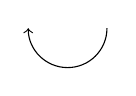
\begin{tikzpicture}[baseline=(A), scale=0.5]
			\coordinate (A) at (0, -0.5);
			\draw[<-] (0, 0) arc[radius=1, start angle=180, end angle=360];
		\end{tikzpicture} \; , \quad
		\mathrm{coev}_X := X \times
		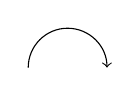
\begin{tikzpicture}[baseline=(A), scale=0.5]
			\coordinate (A) at (0, 0.2);
			\draw[->] (0, 0) arc[radius=1, start angle=180, end angle=0];
		\end{tikzpicture} \; .
	\end{gather*}
	\begin{itemize}
		\item As in the reference above, the definition of $n\dcate{Cob}$
		already incorporates the bijection
		% segment-id: o014.li2.chapter9.duality-examples-a.q012
		\begin{align*}
			\Hom_{n\dcate{Cob}}(X, Y) & \xleftrightarrow{1:1} \Hom_{n\dcate{Cob}}\left( \emptyset, X^* \sqcup Y\right) \\
			& = \left\{ W: \text{oriented with boundary, together with data}\; \partial W \rightiso X^* \sqcup Y \right\} / \sim .
		\end{align*}
		\item The dual of a morphism, that is, of a cobordism, simply reverses
		$\partial W\rightiso X^*\sqcup Y$ to
		$\partial W\rightiso(Y^*)^*\sqcup X^*$.
		\item Trace and dimension take values in
		% segment-id: o014.li2.chapter9.duality-examples-a.q013
		\[ \End_{n\dcate{Cob}}(\emptyset)=
		\{\text{compact closed manifolds of dimension }n\}/\sim . \]
		\item By the description of $\mathrm{ev}_X$ and $\mathrm{coev}_X$
		above, taking the trace of $f\in\End_{n\dcate{Cob}}(X)$ amounts to
		gluing together the two $X$-ends of the cobordism $f$. Since the
		identity morphism $\identity_X$ corresponds to the trivial cobordism
		$X\times[0,1]$, we obtain
		% segment-id: o014.li2.chapter9.duality-examples-a.q014
		\[ \dim X = X \times
		
\begin{tikzpicture}[baseline=(O), scale=0.5]
			\coordinate (O) at (0, -0.25);
			\draw (0, 0) circle[radius=1];
		\end{tikzpicture} \; . \]
	\end{itemize}

	For $n\dcate{Cob}$, the various diagrams introduced in
	\S\ref{sec:monoidal-dual} acquire literal meaning. Here the method and the
	objects share the same geometric substance.
\end{example}
